\section{Installing PGP on Ubuntu}

We will use the Ubuntu Software Centre for installing PGP (Enigmail and
accessories). First open the Ubuntu Software Center through the Unity
menu by typing `software' into the Unity search area

\begin{figure}[htbp]
\centering
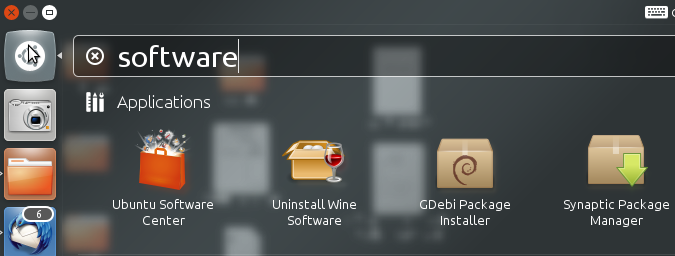
\includegraphics{pgp_ubuntu_inst_1.png}
\caption{PGP Install}
\end{figure}

Click on the `Ubuntu Software Center'.

Type into the search field `Enigmail' and search results should be
returned automatically:

Highlight the Enigmail item (it should be highlighted by default) and
click `Install' and you will be asked to authenticate the installation
process.

\begin{figure}[htbp]
\centering
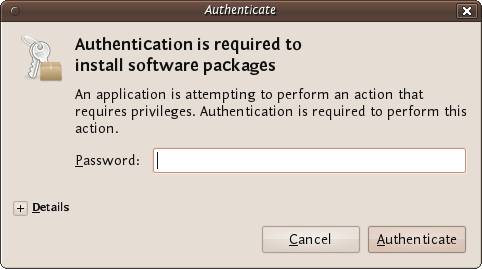
\includegraphics{pgp_ubuntu_inst_2.png}
\caption{PGP Install}
\end{figure}

Enter your password and click `Authenticate'. The installation process
will begin.

When the process is completed you get very little feedback from Ubuntu.
The progress bar at the top left disappears. The `In Progress' text on
the right also disappears. Enigmail should now be installed.
